% !TEX TS-program = pdflatex
% !TEX encoding = UTF-8 Unicode

% This is a simple template for a LaTeX document using the "article" class.
% See "book", "report", "letter" for other types of document.

\documentclass[11pt]{article} % use larger type; default would be 10pt

\usepackage[utf8]{inputenc} % set input encoding (not needed with XeLaTeX)

%%% Examples of Article customizations
% These packages are optional, depending whether you want the features they provide.
% See the LaTeX Companion or other references for full information.

%%% PAGE DIMENSIONS
\usepackage{geometry} % to change the page dimensions
\geometry{a4paper} % or letterpaper (US) or a5paper or....
% \geometry{margin=2in} % for example, change the margins to 2 inches all round
% \geometry{landscape} % set up the page for landscape
%   read geometry.pdf for detailed page layout information

\usepackage{graphicx} % support the \includegraphics command and options
\graphicspath{{./images/}}

% \usepackage[parfill]{parskip} % Activate to begin paragraphs with an empty line rather than an indent

%%% PACKAGES
\usepackage{booktabs} % for much better looking tables
\usepackage{array} % for better arrays (eg matrices) in maths
\usepackage{paralist} % very flexible & customisable lists (eg. enumerate/itemize, etc.)
\usepackage{verbatim} % adds environment for commenting out blocks of text & for better verbatim
\usepackage{subfig} % make it possible to include more than one captioned figure/table in a single float
% These packages are all incorporated in the memoir class to one degree or another...
\usepackage{mcode}
\usepackage{appendix}
\usepackage{amsmath}

%Matrix spacing
\makeatletter
\renewcommand*\env@matrix[1][\arraystretch]{%
  \edef\arraystretch{#1}%
  \hskip -\arraycolsep
  \let\@ifnextchar\new@ifnextchar
  \array{*\c@MaxMatrixCols c}}
\makeatother

%Paragraph spacing
\newcommand{\myparagraph}[1]{\paragraph{#1}\mbox{}\\}

%%% HEADERS & FOOTERS
\usepackage{fancyhdr} % This should be set AFTER setting up the page geometry
\pagestyle{fancy} % options: empty , plain , fancy
\renewcommand{\headrulewidth}{0pt} % customise the layout...
\lhead{}\chead{}\rhead{}
\lfoot{}\cfoot{\thepage}\rfoot{}

%%% SECTION TITLE APPEARANCE
\usepackage{sectsty}
\allsectionsfont{\sffamily\mdseries\upshape} % (See the fntguide.pdf for font help)
% (This matches ConTeXt defaults)

%%% ToC (table of contents) APPEARANCE
\usepackage[nottoc,notlof,notlot]{tocbibind} % Put the bibliography in the ToC
\usepackage[titles,subfigure]{tocloft} % Alter the style of the Table of Contents
\renewcommand{\cftsecfont}{\rmfamily\mdseries\upshape}
\renewcommand{\cftsecpagefont}{\rmfamily\mdseries\upshape} % No bold!

%%% END Article customizations

%%% The "real" document content comes below...

\title{Mars 2040 Optimization: Assignment 1, Section B}
\author{Eric D. Ward, Parker D. Vascik, Samuel Wald}
%\date{} % Activate to display a given date or no date (if empty),
         % otherwise the current date is printed 

\begin{document}
\maketitle
%%%%%%%%%%%%%%%%%%%%%%%%%%%%%%%%%%%%
%2-page Project Proposal
%%%%%%%%%%%%%%%%%%%%%%%%%%%%%%%%%%%%
\section{Project Proposal}
\subsection{Project Introduction}
Our team has decided to do optimization on the Mars 2040 project that Eric worked on in Spring 2015 as the SDM term project.  This project generated a model of a Mars outpost architecture including the Transportation Logistics, Surface Habitation, ISRU and Exploration aspects.  The model was run through a Tradespace exploration to identify architectures that minimized the IMLEO (initial mass to low-earth orbit, i.e. the total payload launched from the Earth surface each synodic period) while attempting to maximize the \'Scientific Value\' as defined as the crew-hours per synodic period available for exploration and research, multiplied by a rank scoring of the landing sites based on an independant study performed early on in the term.

We only have one modification to the model currently planned; to make a small improvement on the utility metric for this project.  Instead of using the more subjective site scoring from the SDM term project, we will formalize the utility as suggested by Ward et. al.\cite{util} to consider quantitative scientific value.

Since the tradespace exploration has already been performed, we will focus this project on more in depth aspects. We will re-run the tradespace exploration with the improved utility metric on the same design space as setup by the SDM term project. From that point, we will select and baseline the architectures in the fuzzy pareto-optimal region, as defined by Smaling and deWeck\cite{fuzzy}.  This should give us approximately 300 baseline architectures. as the starting point for our optimization.

The first portion of our optimization will focus on technology road-mapping.  We will convert some of the parameters in existing model into design variables, based on the possibilities for technological development. For example, we might take the $LOX/LH_2 I_{sp}$ from a parameterized 448 [seconds] and turn it into a variable across the range of $(448,480)$ that we could correlate with a development cost estimate for the improvement in $I_{sp}$.  Once we do this for multiple technologies, we can run an optimization of development spending across the portfolio of technologies for the baselined architectures and determine where the money would be best spent in order to improve the future exploration campaign.

If the first portion goes well, and time permits, we would also like to investigate the build-up campaign as well.  With a baselined technology capability roadmap, we could run through the 300 candidate architectures from a null-infrastructure to the full 20 person outpost, looking for a sub-game perfect campaign that would optimize not only the steady-state re-supply missions, but the entire campaign from the beginning.

\subsection{Formal Problem Statement}
To optimize the improvements to a campaign to setup a permanently inhabited outpost on the surface of Mars from a technology development budget, by altering the design variables associated with technological performance across pre-selected architectures, using systems design optimization methodoligies. 
\subsection{Design Variables, Parameters, Constraints, Bounds and Objectives}


\myparagraph{Objective Function}

maximize $J(\mathbf{u})$ (Campaign Utility)

\myparagraph{Design Variables}
\begin{equation*}
\mathbf{x}=
\begin{bmatrix}[1.5]
Isp_{LH_2}\\
Isp_{NTR}\\
\alpha_{ISRU}\\
\end{bmatrix}
=
\begin{bmatrix}[1.5]
LH_2 Isp\\
Nuclear Thermal Rocket Isp\\
ISRU efficiency\\

\end{bmatrix}
\end{equation*}



\myparagraph{Parameters}

More text.

\myparagraph{Constraints}

More text.

\myparagraph{Bounds}

More text.

%%%%%%%%%%%%%%%%%%%%%%%%%%%%%%%%%%%%
%Model Description
%%%%%%%%%%%%%%%%%%%%%%%%%%%%%%%%%%%%
\clearpage
\section{$N^2$ Diagram}

More text.

\section{Block Diagram}
Figure \ref{fig:m2040block} shows the model layout from the Mars 2040 SDM term project from the Spring term of 2015.  This will be the starting point for our model for MSDO.  Throughout the semester, the model may require some modifications based on the changes in scope (going from a tradespace exploration to a development optimization.) However, we feel like this arrangement does a good job setting up the project, and the changes will not likely require massive rearrangements.
\begin{figure}
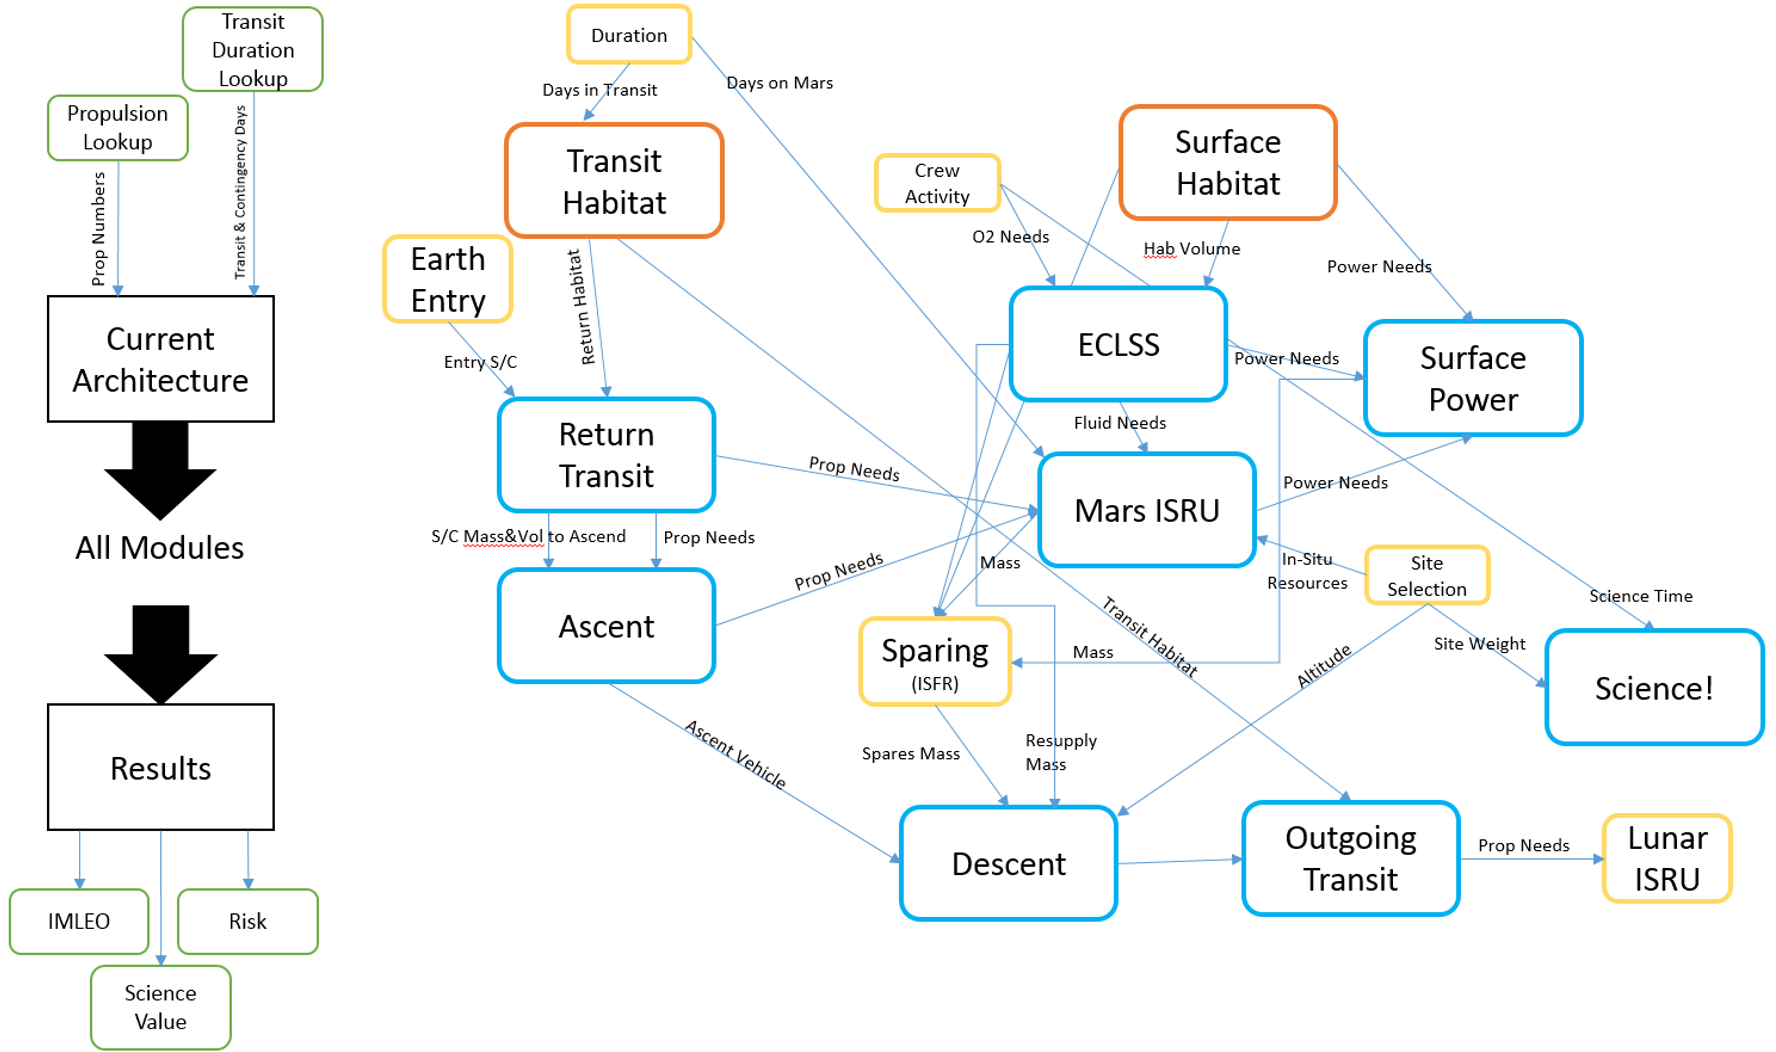
\includegraphics[width=\textwidth]{M2040Block}
\label{fig:m2040block}
\caption{Block Diagram of Model from the Mars2040 Project Spring 2015}
\end{figure}

\clearpage
\begin{thebibliography}{1}
\bibitem{util} Eric D. Ward, Ryan R. Webb, Olivier L. deWeck, {\em A Method to Evaluate Architectural Comparisons for a Campaign to Explore the Surface of Mars}. Manuscript submitted for publication, Acta Astronautica. 2016.
\bibitem{fuzzy}Smaling R., de Weck O., "Assessing Risks and Opportunities of Technology Infusion in System Design", {\em Systems Engineering}, 10 (1), 1-25, Spring 2007
\end{thebibliography}

\clearpage
\begin{appendices}
\section{Master Table}

\end{appendices}

\end{document}
